\section{The \tool{} System}
\label{sec:architecture}
\label{sec:principles}

\tool{} consists of two separately installable packages (Figure~\ref{fig:overview}). \texttt{tsfm\_benchmark}
generates, audits, seals and validates corpora; \texttt{tsfm\_lens} loads checkpoints through adapters, runs a gated
pipeline of analysis stages and renders the report. This section describes the parts that make cross-model
measurements valid; implementation details and usage are in Appendix~\ref{sec:usage}.

\subsection{Design principles}

Each principle below is enforced in code as a gate, a refusal or a test, so that a measurement that cannot be trusted
is withheld with a stated reason rather than reported.
\begin{description}[leftmargin=1.2em,font=\normalfont\bfseries,itemsep=1pt]
\item[P1. Ground truth by construction.] Every probe is first validated on a case whose answer is known.
\item[P2. Alignment is measured, not declared.] Token spans are measured from impulse responses, and cross-model
  analysis happens only on a common time axis.
\item[P3. Causal claims need a null, a reach control and a same-seed baseline.] Every intervention is compared with a
  random intervention of matched size on the same series, and sampled models are seeded identically in compared calls.
\item[P4. The series is the unit of inference.] All intervals and $p$-values resample whole series.
\item[P5. Explore, then confirm once.] Dev results are exploratory; registered claims are tested once on a sealed
  split.
\item[P6. Every claim is typed, and failures are loud.] Each finding carries an evidence class and a generated caveat,
  and unsupported analyses are skipped with a rendered reason.
\end{description}
The evidence classes are \ev{behavioral} (input--output only), \ev{descriptive}, \ev{illustrative},
\ev{geometric} (representational similarity), \ev{linear-translatable} (one representation linearly predicts
another beyond an input baseline), \ev{causal within-model} (an intervention changes the forecast beyond a null) and
\ev{held-out confirmed} (a registered claim replicated on the sealed split). A \ev{predictive} class marks internals
that forecast a model's error without being shown to cause it.

\subsection{Controlled benchmark generation}
\label{sec:benchmark}
\label{sec:layout}

Real data enter the benchmark only as leakage references, for realism calibration and as raw material for explicitly
labeled generators. Generators come in two tiers. The \emph{synthetic} tier touches no real data and has exact ground
truth. Its \texttt{parametric} generator is additive (trend, multiple seasonalities, AR noise, changepoints,
anomalies, random walk, intermittency and heteroskedasticity), and \texttt{random\_parametric} draws a recipe from one
of eight frozen archetypes. The \emph{real-derived} tier (\texttt{mixture}, \texttt{block\_bootstrap}
\citep{kunsch1989block} and \texttt{sequential\_par}) inherits its source distribution and has only attributional
ground truth. Because ``free of leakage'' and ``realistic'' pull in opposite directions, every sample carries its tier
label and every analysis can be split by tier.

Every sample passes a two-stage leakage gate against the Monash archive \citep{godahewa2021monash}, a cheap prefilter
followed by banded DTW \citep{sakoe1978dtw}, and a cross-split near-duplicate check. Dev and private splits use disjoint
seed ranges mixed with SHA-256. Every sample is hashed, so that loading a sealed split with verification detects any
change, and fresh private \emph{epochs} are minted by striding the seed space. A validation package measures redundancy
by shape matching and diversity in the catch22 feature space \citep{lubba2019catch22}, using the participation-ratio
dimension \citep{gao2017pr} and nearest-neighbor tails rather than a 2-D embedding. It also tests dev/private
exchangeability with an energy-distance test \citep{szekely2013energy} and per-feature TOST equivalence
\citep{schuirmann1987tost}.

Two perturbation families are built in. Nine structured \emph{corruptions} (noise, detrend, deseasonalize, frequency
shift, level shift, spike, smooth, warp and dropout) drive the perturbation analysis of Section~\ref{sec:l3}.
\emph{Generator counterfactuals} move one generative parameter along a dose ladder with every random draw held fixed; dose
1.0 must reproduce the original series bit-exactly, an identity test that caught a real replay bug (\fid{BM-05}).

\subsection{Model adapters and capability tiers}
\label{sec:adapters}

A model enters through an adapter that exposes loading, a \texttt{predict} method returning point and quantile
forecasts in the original scale, the underlying module, input preparation, a forward pass and the time span of each
token. The adapter's \emph{capability tier} is derived from the methods it implements rather than declared: 0 (black
box), 1 (observable hidden states with token spans), 2 (steerable, so patching is possible) and 3 (decomposable
attention). Stages above a model's tier are skipped with the missing method named in the report. A missing capability
is a fact about the adapter; a measured failure of time localization is a fact about the model, and routes it to
behavioral analysis only.

New checkpoints can use a zero-code adapter for Hugging Face models, which discovers layers, measures token spans and
refuses rather than guesses. Its span discovery reproduces the spans of all six hand-written adapters exactly and
recovers Timer's 96-step tokens from measurement alone (\fid{MP-01}). Two of the seven models studied here use it.

\subsection{Time alignment across architectures}
\label{sec:alignment}

Each token's time span is measured from its impulse response, gated on peak-to-pedestal contrast and contiguity. Given
spans $I_j$ and windows $W_w=[wL,(w+1)L)$, with $L=32$ by default, tokens are overlap-pooled:
\begin{equation}
  P_{wj} = \frac{|I_j \cap W_w|}{\sum_{j'} |I_{j'} \cap W_w|}, \qquad \tilde h_w = \sum_j P_{wj}\, h_j .
  \label{eq:pooling}
\end{equation}
Every cross-model analysis runs on the resulting $[\text{series},\text{window},\text{dim}]$ tensors
(Figure~\ref{fig:alignment}), and an empty window raises an error rather than yielding a zero row. During extraction an
\emph{alignment gate} injects an impulse into each window and checks, layer by layer, that the matching pooled window
responds most. Hits are normalized by their attainable ceiling, because a 96-step token pooled onto 32-step windows can
reach at most one third (\fid{MP-02}), and the impulse amplitude is calibrated per checkpoint and context length.

\begin{figure}[tb]
\centering
\begin{tikzpicture}[x=0.36mm,y=5.5mm,font=\scriptsize]
  \foreach \row/\name/\w/\col in {3/TimesFM (32)/32/tfm, 2/{Chronos-2, Sundial, Bolt (16)}/16/ctwo, 1/Chronos-T5 (1)/4/gray, 0/Timer (96)/96/sun}{
    \node[anchor=east] at (-4,\row) {\name};
    \pgfmathtruncatemacro{\n}{288/\w-1}
    \foreach \k in {0,...,\n}{
      \draw[fill=\col!25, draw=\col!80!black, line width=0.3pt] (\k*\w,\row-0.32) rectangle ({(\k+1)*\w},\row+0.32);
    }
  }
  \foreach \k in {0,...,8}{
    \draw[thick, accent] (\k*32,-1.0) rectangle ({(\k+1)*32},-0.45);
    \node[font=\tiny] at (\k*32+16,-0.72) {$W_{\k}$};
  }
  \node[anchor=east] at (-4,-0.72) {common windows ($L{=}32$)};
  \draw[-{Stealth}, accent] (80,-0.3) -- (80,-0.02);
  \draw[decorate,decoration={brace,amplitude=3pt,mirror}] (0,-1.15) -- (288,-1.15) node[midway,below=3pt] {time (first 288 context steps)};
\end{tikzpicture}
\caption{Time alignment. Tokens cover measured spans of different widths (Chronos-T5's one-step tokens are drawn
in groups of four); Equation~\eqref{eq:pooling} pools them onto common windows.}
\label{fig:alignment}
\end{figure}

\subsection{The stage pipeline and the report}
\label{sec:stages}
\label{sec:report}

An analysis is a pipeline of 19 stages that write typed artifacts (Figure~\ref{fig:stages}). Each stage declares the
configuration keys it depends on, and these are fingerprinted, so a changed setting invalidates exactly the dependent
cached artifacts. Three gates record their decisions and the report names them as skip reasons: the \emph{tier} gate,
the \emph{run-shape} gate, which drops comparison stages when only one model is given, and the \emph{routing} gate for
models that are not time-localized. Every intervention goes through a single patching primitive, which raises an error
if the model silently splits a batch.

\begin{figure}[tb]
\centering
\begin{tikzpicture}[
  node distance=2.2mm and 2.2mm,
  st/.style={draw, rounded corners=1.5pt, font=\scriptsize\sffamily, minimum width=13mm, minimum height=5.5mm, fill=white},
  arr/.style={-{Stealth[length=1.4mm]}, gray!70!black},
  band/.style={rounded corners=3pt, inner sep=3pt},
  blab/.style={font=\scriptsize\bfseries, anchor=west}]
  \node[st] (corpus) {corpus};
  \node[st, right=of corpus] (extract) {extract};
  \node[st, right=of extract] (budget) {budget};
  \node[st, right=of budget] (frontend) {frontend};
  \node[st, right=of frontend] (screen) {layer\_screen};
  \node[st, below=5mm of corpus] (l0) {l0};
  \node[st, right=of l0] (internals) {internals};
  \node[st, right=of internals] (lens) {lens};
  \node[st, below=5mm of l0] (l1) {l1};
  \node[st, right=of l1] (l2) {l2};
  \node[st, right=of l2] (cluster) {cluster};
  \node[st, below=5mm of l1] (l3) {l3};
  \node[st, right=of l3] (attention) {attention};
  \node[st, right=of attention] (sae) {sae};
  \node[st, right=of sae] (concepts) {concepts};
  \node[st, below=5mm of l3] (exemplars) {exemplars};
  \node[st, right=of exemplars] (register) {register};
  \node[st, right=of register] (confirm) {confirm};
  \node[st, right=of confirm, fill=accent!15] (report) {report};
  \begin{scope}[on background layer]
    \node[band, fill=gray!10, fit=(corpus)(screen)] (b1) {};
    \node[band, fill=tfm!10, fit=(l0)(lens)] (b2) {};
    \node[band, fill=ctwo!10, fit=(l1)(cluster)] (b3) {};
    \node[band, fill=sun!12, fit=(l3)(concepts)] (b4) {};
    \node[band, fill=accent!10, fit=(exemplars)(report)] (b5) {};
  \end{scope}
  \node[blab] at ($(b1.east)+(2mm,0)$) {setup \& cost};
  \node[blab, align=left] at ($(lens.east)+(4mm,0)$) {behavioral / descriptive\\[-1pt]{\scriptsize\rmfamily\mdseries L0 accuracy, depth profile, lens}};
  \node[blab, align=left] at ($(cluster.east)+(4mm,0)$) {geometric / linear-translatable\\[-1pt]{\scriptsize\rmfamily\mdseries L1 CKA/RSA, L2 stitching, clusters}};
  \node[blab, align=left] at ($(b4.east)+(2mm,0)$) {causal within-model\\[-1pt]{\scriptsize\rmfamily\mdseries patching, heads, SAE ablation}};
  \node[blab, align=left] at ($(b5.east)+(2mm,0)$) {held-out confirmed};
  \draw[arr] (b1.south) -- (b2.north -| b1.south);
  \draw[arr] (b2.south -| b1.south) -- (b3.north -| b1.south);
  \draw[arr] (b3.south -| b1.south) -- (b4.north -| b1.south);
  \draw[arr] (b4.south -| b1.south) -- (b5.north -| b1.south);
\end{tikzpicture}
\caption{The 19-stage pipeline, grouped by the strongest evidence class each group can produce. Gates
(tier, run shape, routing, configuration fingerprints) skip a stage per model with a rendered reason; only
\texttt{confirm}, on the sealed private split, produces \ev{held-out confirmed} evidence.}
\label{fig:stages}
\end{figure}

The deliverable is one self-contained HTML file, designed so that a reader without interpretability training can
follow it while an expert can audit every number (Figure~\ref{fig:report}). Its sections pose plain questions, such as
``Is the comparison fair?'' or ``What causally drives the forecast?''. Each stage opens with a card stating its
question, its method, what good and bad results look like and what it cannot show, and every figure carries a caption
and an expandable explanation. The summary scorecard is computed from the artifacts by printed rules, with no model
names hard-coded: each row shows a value, the reference it is compared with (a null, floor, ceiling or baseline) and the
rule that yields the verdict. Every claim is a typed record with its evidence class, a plain-language sentence and a
generated caveat. Skipped stages show the gate's reason, failed sections render visibly, and a multiplicity ledger flags
correction families that cannot reach significance.

\begin{figure}[tb]
\centering
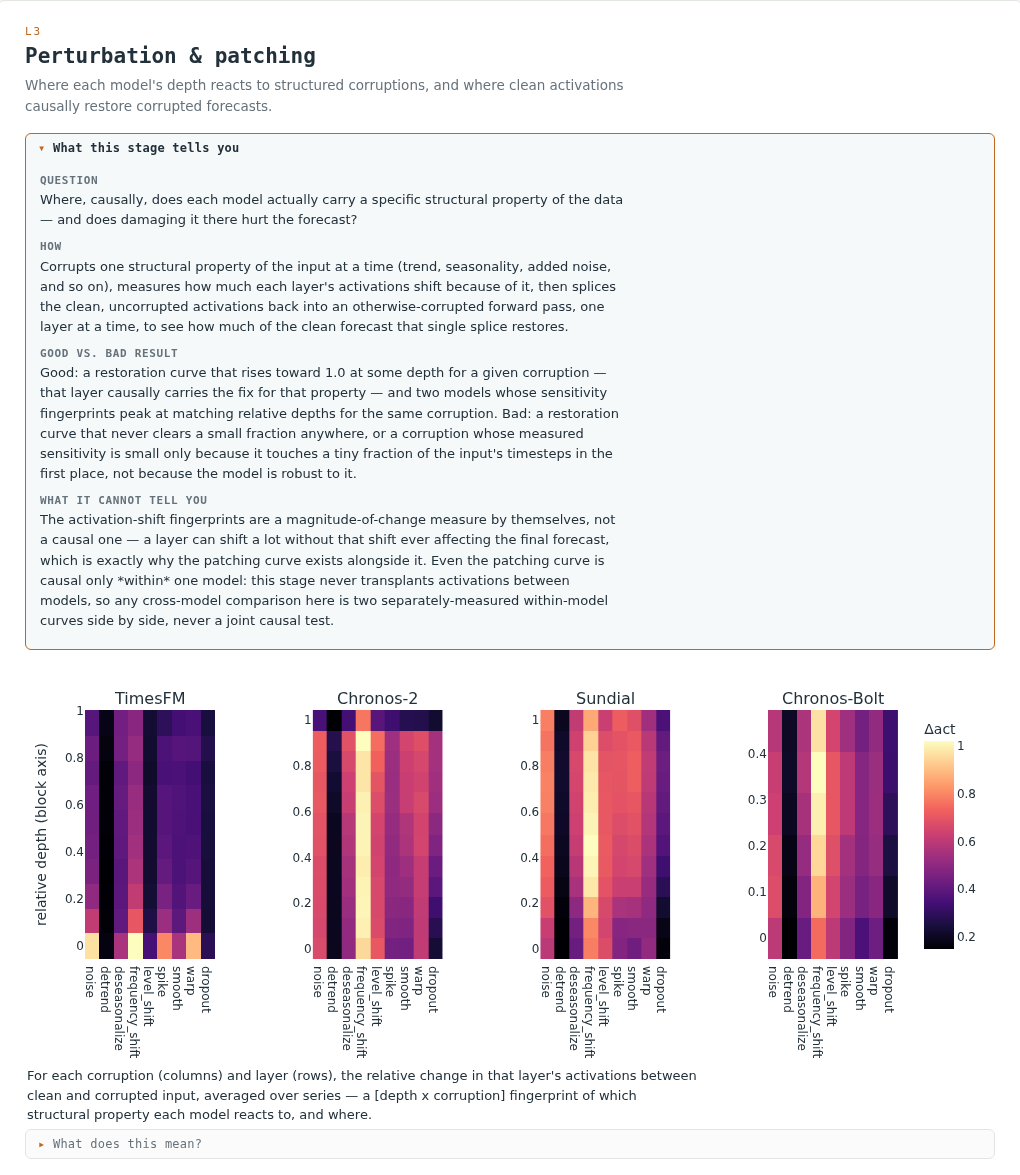
\includegraphics[width=0.42\textwidth]{figures/report_l3_crop.png}
\caption{Excerpt of the generated report (perturbation section of the seven-model example report,
\repodir{examples/panel7_v2}). The stage card states the question, method, how to read good and bad results and the
limitation, above the per-model corruption-sensitivity fingerprints.}
\label{fig:report}
\end{figure}
